\documentclass[11pt]{article}
\usepackage{geometry}                % See geometry.pdf to learn the layout options. There are lots.
\geometry{letterpaper}                   % ... or a4paper or a5paper or ... 
%\geometry{landscape}                % Activate for for rotated page geometry
%\usepackage[parfill]{parskip}    % Activate to begin paragraphs with an empty line rather than an indent
\usepackage{graphicx}
\usepackage{amssymb}
\usepackage{epstopdf}
\usepackage{tikz}
\usetikzlibrary{automata,positioning}       
\usepackage{listings}
\lstset
{ %Formatting for code in appendix
    language = C,
    basicstyle=\footnotesize,
    numbers=left,
    stepnumber=1,
    showstringspaces=false,
    tabsize=1,
    breaklines=true,
    breakatwhitespace=false,
}   
\DeclareGraphicsRule{.tif}{png}{.png}{`convert #1 `dirname #1`/`basename #1 .tif`.png}

\title{Conceptual Design}
\author{Aneesh Malhotra, Ryan Thomas, Mohammed Nur, Sohail Iqbal, Gerson Dalton}
%\date{}                                           % Activate to display a given date or no date

\begin{document}
\maketitle

\section{Introduction}
This project will build upon a previous ECE 492 project \textit{FPGA Enhanced Wireless Sensor Node for IoT Applications}. The previous project constructed a motion-triggered wireless sensor node that takes snapshots and sends them over ZigBee to a gateway device. The gateway then sends the image to a Dropbox cloud. This entire process was enhanced by elliptic curve cryptography which was implemented using an Actel Igloo Nano FPGA. 

\section{Conceptual Design}

\subsection{Application} 

\subsubsection{Camera Module}

\begin{itemize}
\item The camera being used is the ArduCAM v5 5MP camera with night-vision capability (\$21).
\item The camera module will be controlled by the MSP430 through $I^2C$ for instructions, and $SPI$  for the images.
\end{itemize}

\subsubsection{Android Development}

\begin{itemize}
\item The Android app is used to receive photos via the Dropbox cloud from the gateway.
\item The app will allow the user to manually request a snapshot.
\item The app will setup a private connection via ECC, and allow the user to update the private key of the user. 
\item The app will be updated to deliver OTA updates via the dropbox cloud.
\end{itemize}

\subsection{Dropbox Cloud}
\begin{itemize}
\item Used to store updates and photos, as per the user's request.
\end{itemize}

\subsection{Gateway}
\begin{itemize}
\item Uses a BeagleBone Black to connect the node to the Dropbox cloud.
\item Communicates to the network via Ethernet, which is secured by transport layer security.
\item Communicates with the node via the ZigBee protocol, which is secured through AES.
\end{itemize}


\subsection{Node}
\subsubsection{FPGA}
\begin{itemize}
\item The Actel Igloo Nano will be used for securing the user's phone to the node.  
\item The FPGA will use elliptic curve cryptography, which uses smaller private keys than alternatives, allowing for more efficient use of memory.
\end{itemize}


 \subsubsection{MSP432}
 \begin{itemize}
 \item Used as a controller for the FPGA, XBee, ArduCAM, and PIR Motion Sensor.
 \item The MSP432 will be initialized by the motion sensor or user input, and send a signal to the ArduCAM to take a snapshot.
 \item The MSP432 will receive the snapshot in JPEG format via SPI, and transmit the image to the XBee via the UART protocol.
 \item The MSP432 will use the key generated by the FPGA to secure this communication with the user.
 \end{itemize}
 

\section*{Schematic}

\begin{figure}[!ht]
\centering
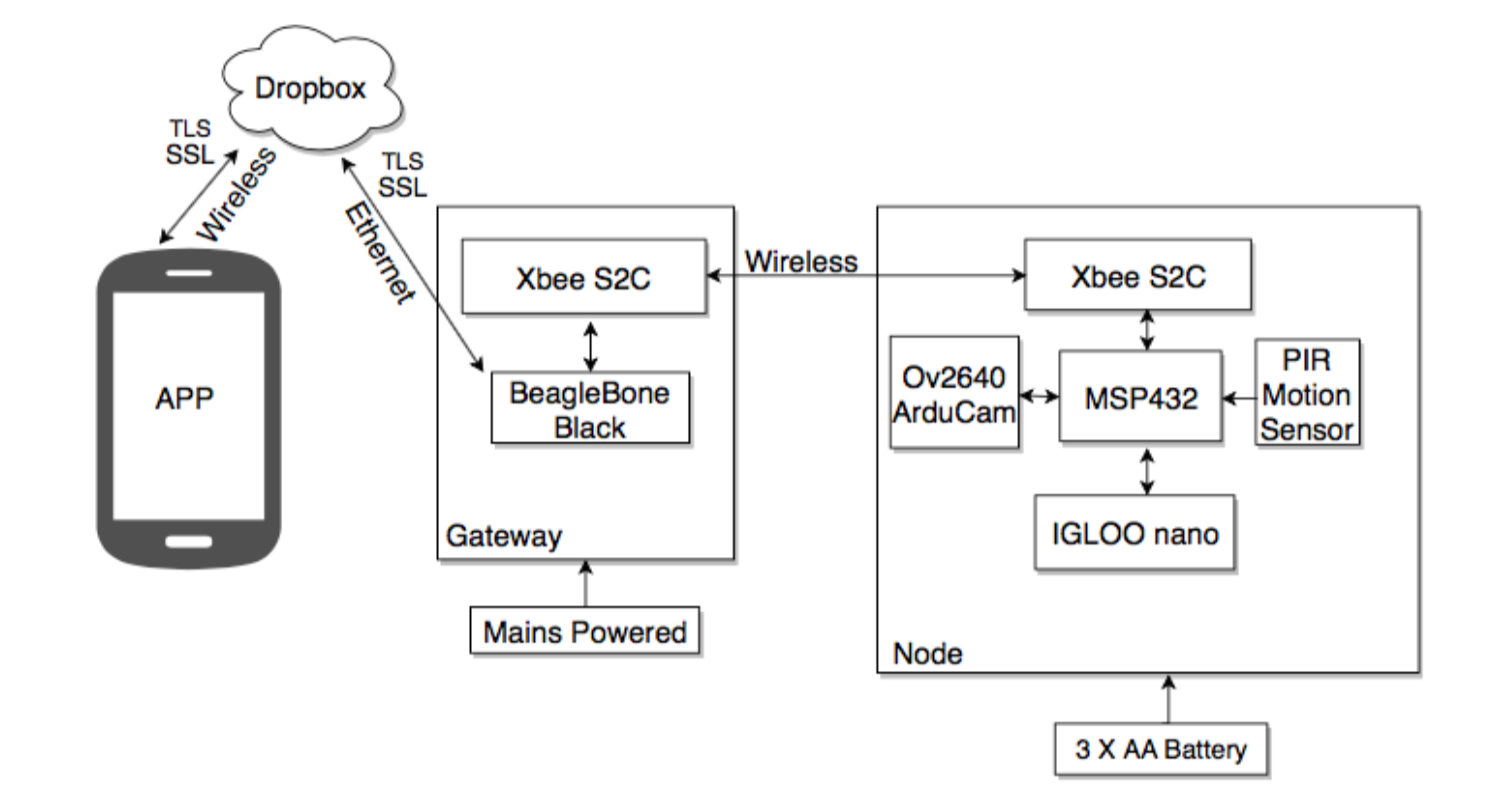
\includegraphics[scale = 0.6]{schematic1.png}
\caption{Top Level Schematic}
\end{figure}

\begin{figure}[!ht]
\centering
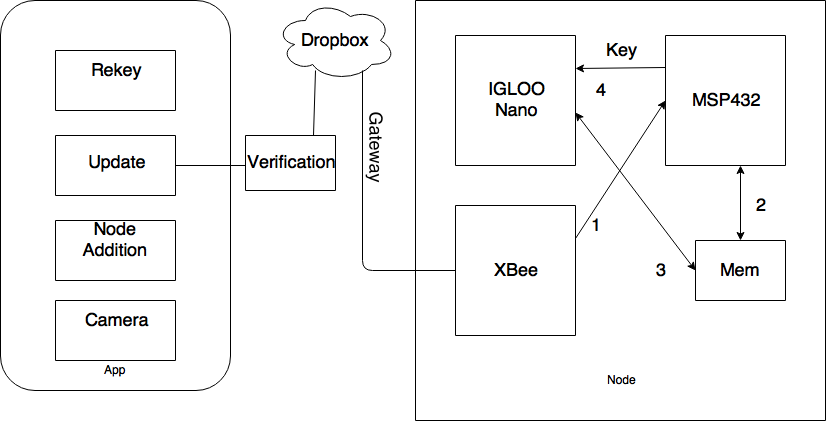
\includegraphics[scale = 0.6]{Diagram1.png}
\caption{Top Level Diagram}
\end{figure}







\end{document}  